\documentclass{article}
\usepackage{amsmath}
\usepackage{mathtext}
\usepackage[english,russian]{babel}
\usepackage[T2A]{fontenc}
\usepackage[utf8]{inputenc}
\usepackage{graphicx}
\graphicspath{{img/}}
\DeclareGraphicsExtensions{.jpg, .png, .pdf}
\begin{document}
\section {Зубчатые передачи. Достоинства, недостатки. Классификация зубчатых передач.}

\section {Кинематика червячной передачи. Параметры червяка и червячного ЗК.}

\section {Конические передачи. Расчет сил и моментов в конической передаче.}

\section {Косозубые передачи. Расчет сил и моментов в косозубой передаче.}

\section {Люфтовыбирающее колесо. Методика расчета.}

\section {Механические передачи. Примечание. Основные характеристики передач.}

\underline{Механические передачи}  -- механизмы, предназначенные для передачи и преобразования 
энергии, моментов сил, скоростей от ведущего к ведомому элементу.

\underline{Применяются}, когда необходимо:
\begin{enumerate}
	\item Преобразование движения:
	\begin{enumerate}
		\item Из вращения в перемещение
		\item Из врадения в вращение
		\itemИз вращения в перемещние по опр-му закону
	\end{enumerate}
	\item Изменение скорости в саомй передаче
	\item Управление несколькими потребителями от одного источника
\end{enumerate}

\underline{Основные характеристики передач:}

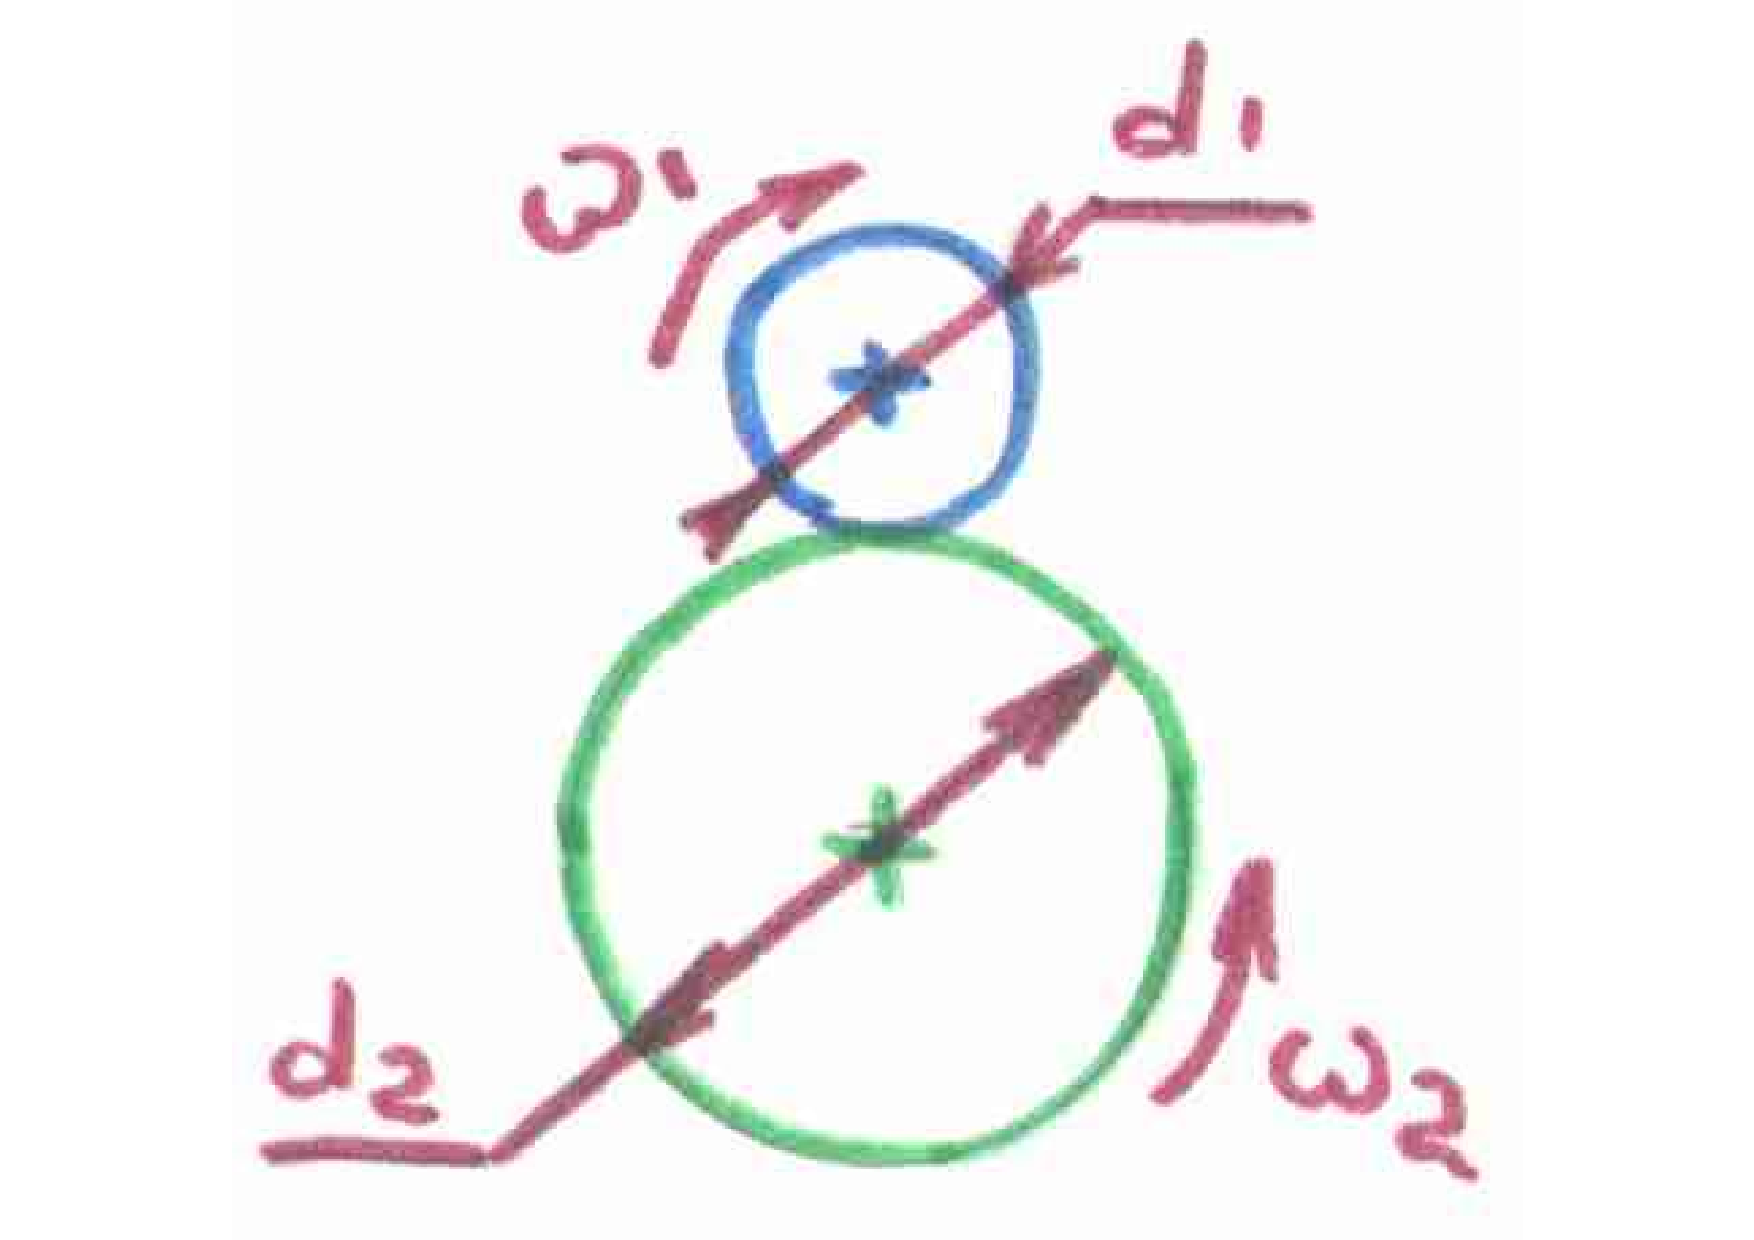
\includegraphics[width = 0.4\textwidth]{6_1}

\begin{enumerate}
	\item Зависимость между входной и выходной величиной $\omega_{вх}$ ($\omega_{выx}$)
	\item Передаточное отношение $i_{1\:2} = \frac{ \frac{d\omega_1}{dt} }{ \frac{d\omega_2}{dt} } = \frac{\omega_1}{\omega_2} = \frac{n_1}{n_2} = \frac{d_2}{d_1} $ -- отношение
	мгновенных скоростей ведущего и ведомого элементов.
	\item  КПД: $\eta = \frac{P_{пол}}{P_{зат}} = \frac{P_{зат} - P_{потерь}}{P_{зат}} = 1 - \frac{P_{потерь}}{P_{зат}} = 1 - \psi_{потерь} $
\end{enumerate}

\section {Основная теорме зацепления. Эвольвента и ее свойства. Параметры зубчатого колеса.}

\underline{Основная теорема зацеплния} 

\section {Отсчетные устройства. Методика расчета.}

\section {Параметры эвольвентного зацепления. Анализ сил и моментов в одноступенчатой зубчатой передаче.}

\section {Подбор двигателя редуктора. Методика расчета.}

\section {Потенциометры. Принцип действия. Методика расчета. Варианты установки на корпус редуктора (чертеж).}

\section {Расчет модуля колес. Расчет на контактную прочность.}

\section {Расчет на точность. Вероятностный метод.}

Допуск на кинематическую погрешность колеса находят как сумму допусков на накопительную
погрешность шага $F_p$ и допуска на погрешность профиля зуба $f_f$:
$$
F_i^{'} = F_p^{'} + f_{f_i}
$$
Допуск на угловую кинематическую погрешность в угловых минутах находят так:
$$
\Delta \varphi_{max, i} = \frac{6.88 \cdot K F_i^{'}}{m z_i} 
$$
Где $K$ - коэффициент фазовой компенсации.

Теперь считаем минимальный допуск на угловую кинематическую погрешность.

\begin{tabular}{cc}
$ \Delta \varphi_{min,i} = \frac{4.88 \cdot K_s F_i^{'}}{m z_i} $ & для 7,8 класса точности \\
$ \Delta \varphi_{min,i} = \frac{4,3 \cdot K_s F_i^{'}}{m z_i} $  & для 5, 6, 9, 10 классов точности
\end{tabular}

Найдем поле рассеивания:
$$
V_i = \varphi_{max, i} - \varphi_{min, i}
$$

Координаты середины поля рассеивания: $E_i = \frac{ \Delta \varphi_{max, i} + \Delta \varphi_{min, i}}{2} $
Суммарная вероятностная кинематическая погрешность:
$$
\Delta \varphi_{i, \Sigma}^{B} = \sum\limits_{j = 1}^{N} \frac{E_{i,j}}{i_j - N} + t_1 \sqrt[2]{\sum\limits_{j = 1}^{N} \left(\frac{V_{i,j}}{i_j - N}\right)^2}
$$
$t_1$ -- коэф-т Стьюдента

\underline{Опр-е погрешностей, вносимых мертвым ходом} 

$$
V_{л, i} = \Delta \varphi_{л, max_j} - \Delta \varphi_{л, min_j}
$$
$$
\Delta \varphi_{л min_j} = \frac{7.33 \cdot j_{n, min}}{m z_j} 
$$
$$
\Delta \varphi_{л max_j} = \frac{7.33 \cdot j_{n, max}}{m z_j} 
$$
$$
E_{л_j} = \frac{ \Delta \varphi_{j \: л \: max} + \Delta \varphi_{j \: л \: min}}{2}
$$
$$
\Delta \varphi_{л}^{Вер} = \sum\limits_{j = 1}^{N} \frac{E_{л \: j}}{i_{j - N}} + t_2 \sqrt[2]{\sum\limits_{j = 1}^{N} \left(\frac{V_{i \: j}}{i_{j - N}} \right)^2}
$$

\section {Расчет на точность. Метод максимум-минимума}

Допуск на кинематическую погршность колеса находят как сумму допусков на накопленную погрешность шага $F_p$
и допуска на погрешность профиля зуба $f_f$
$$
F_{f}^{'} = F_{i\:i} + F_{f\:i}
$$
Допуск на угловую кинематическую погрешность в угловых минутах находят как:
$$
\Delta \varphi_i = \frac{6.88 \cdot F_i^{'}}{m z_i} 
$$
Суммарная кинематическая погрешность:
$$
\Delta \varphi_{i\:o\:\Sigma} = \sum\limits_{j = 1}^{N} \frac{ \Delta \varphi_{i\:j}}{m z_i}
$$
$K_\varphi$ -- коэффициент, учитывающий зависимость кинематической погрешнсоти рассчитываемой передачи от максмального 
угла поворота колеса.

\underline{Опр-е погрешностей вносимых мертвым ходом}

Собственный люфтовые погрешнсоти передачи отнесенные к ведущим колесам (шестерням) каждой пары:
$$
\Delta \varphi_{л \: i} = \frac{7.33 \cdot j_{n\:max\:i}}{m z_i} 
$$
$j_{n\:max}$ -- максимальный боковой зазор
$$
j_{n\:max} = 0.7 \left (E_{HS_1} + E_{HS_2}\right) + \sqrt[2]{0.5\cdot\left(T_{H_1}^2 + T_{H_2}^2\right) + 2 * \left(f_a\right)^2}
$$
$E_{HS_1}$, $E_{HS_2}$ -- наименьшее смещение исходного контура шестерни и колеса
$T_{H_1}, T_{H_2}$ -- допуск на смещение исх. контур шестерни и колеса
$f_a$ -- допуск на отклонение межосевого расстояния
$$
\Delta \varphi_{л\:\Sigma} = \sum\limits_{j=1}^{N-1} \frac{ \Delta \varphi_{л \: i}}{i_{j - N}} 
$$

\section {Сложные передачи. Волновые передачи.}

По конструктивному исполнению различают фрикцонные и зубчатые. Р-м принцип действия фрикционной влонвой передачи

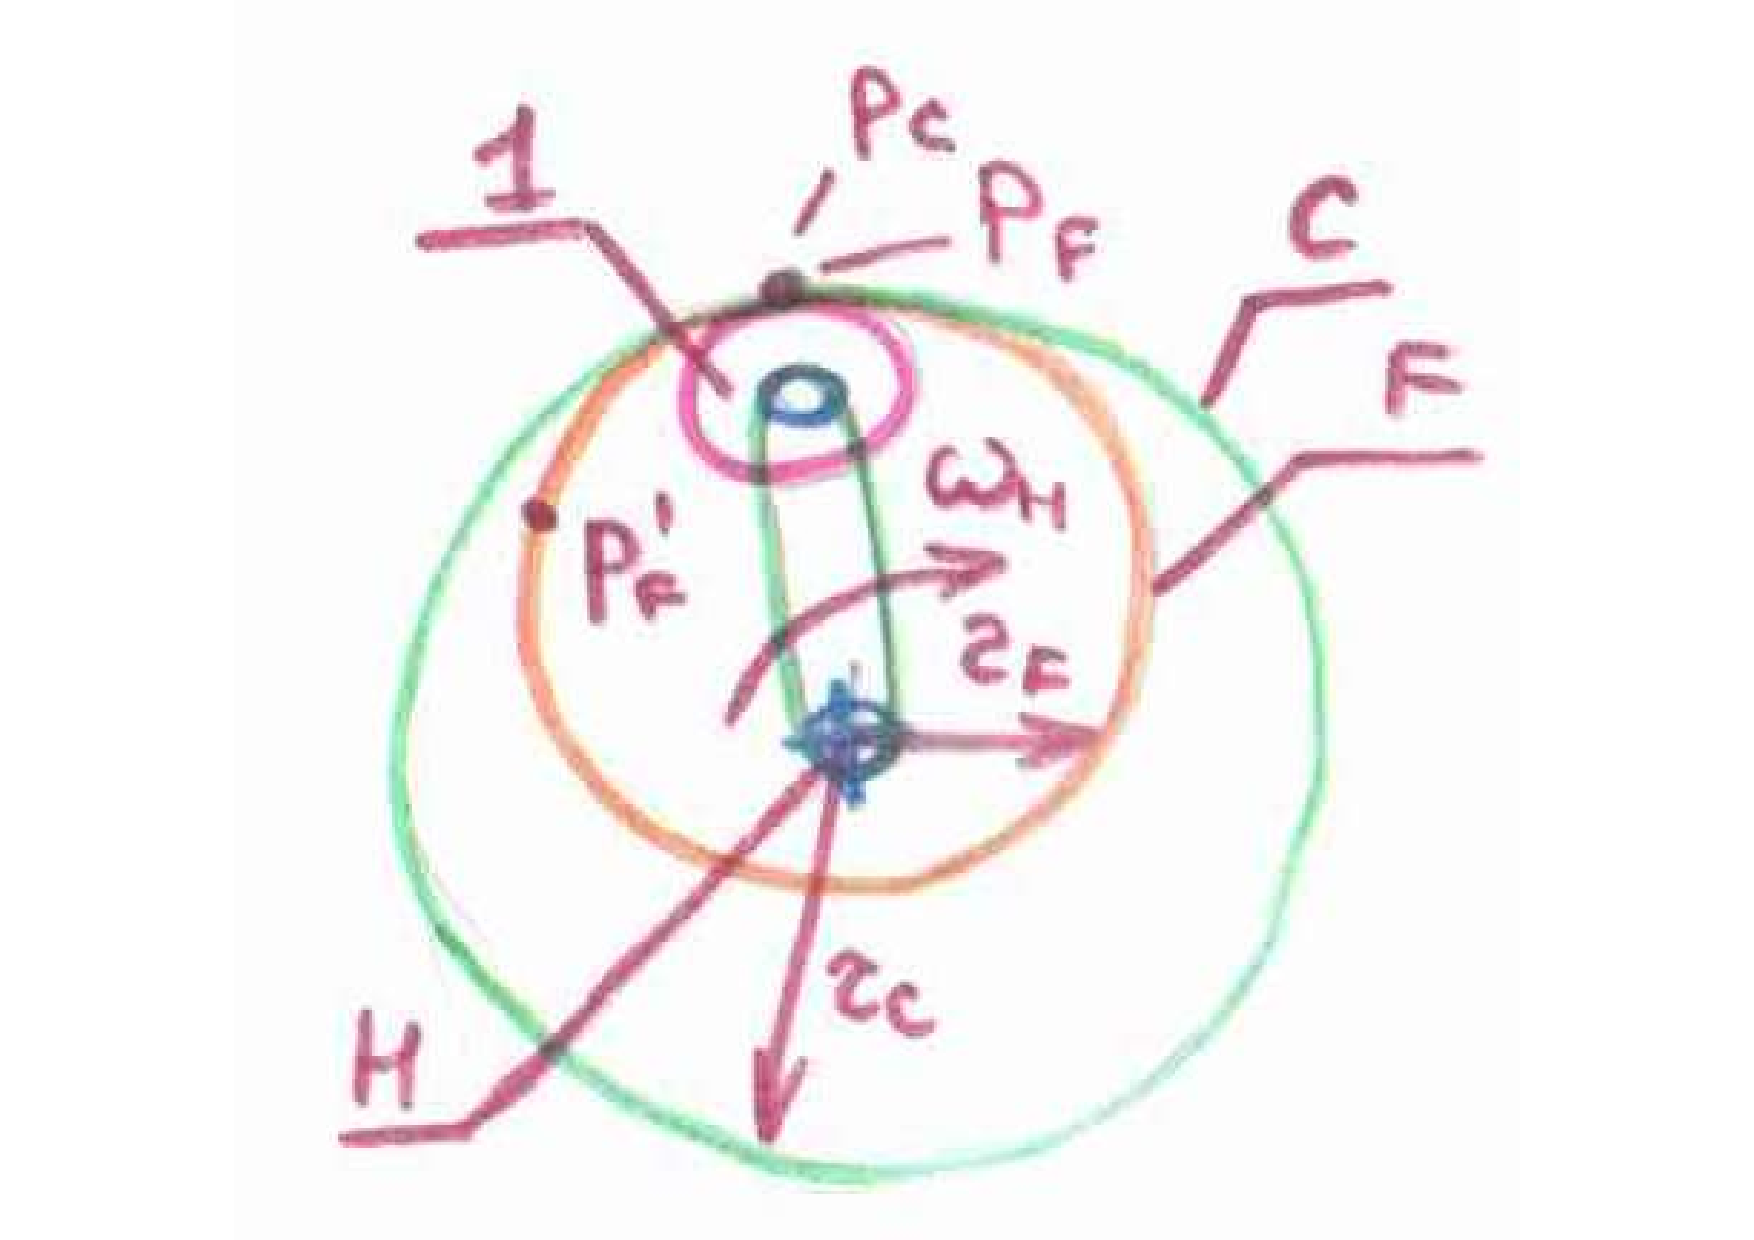
\includegraphics[width = 0.2\textwidth]{15_1}

Внутрь жесткого неподвижного цилиндрического кольца C вставлено гибкое кольцо F? прижатое роликом 1, закрепленным на водиле H
$L_F$ -- длина внутренней окр-ти.
$L_C$ -- длина внешней окр-ти.

При вращении водила по часовой стрелке, внутреннее колесо вращается против часовой стрелки. Считаем, что проскальзывание отсутствует.

За 1 оборот водила гибкое кольцо повернется на небольшой угол, определяемый дугой $\rho_F$ $\rho_F^{'} = L_C - L_F$, посему чем меньше разница длины окружностей, тем меньшеугол поворота внутреннего колеса.

Таким образом, происходит преобразование быстрого вращения водила с угловой скоростью $\omega_H$ в обратное по направлению и замедленное по вражению гибкого вала кольца

$$
i_{HF} = \frac{L_F}{L_C - L_F}  = - \frac{\pi dc}{\pi dc - \pi df} = - \frac{dF}{ \Delta} 
$$
$$
i_{HF} = - \frac{z_F}{z_C - z_F} 
$$

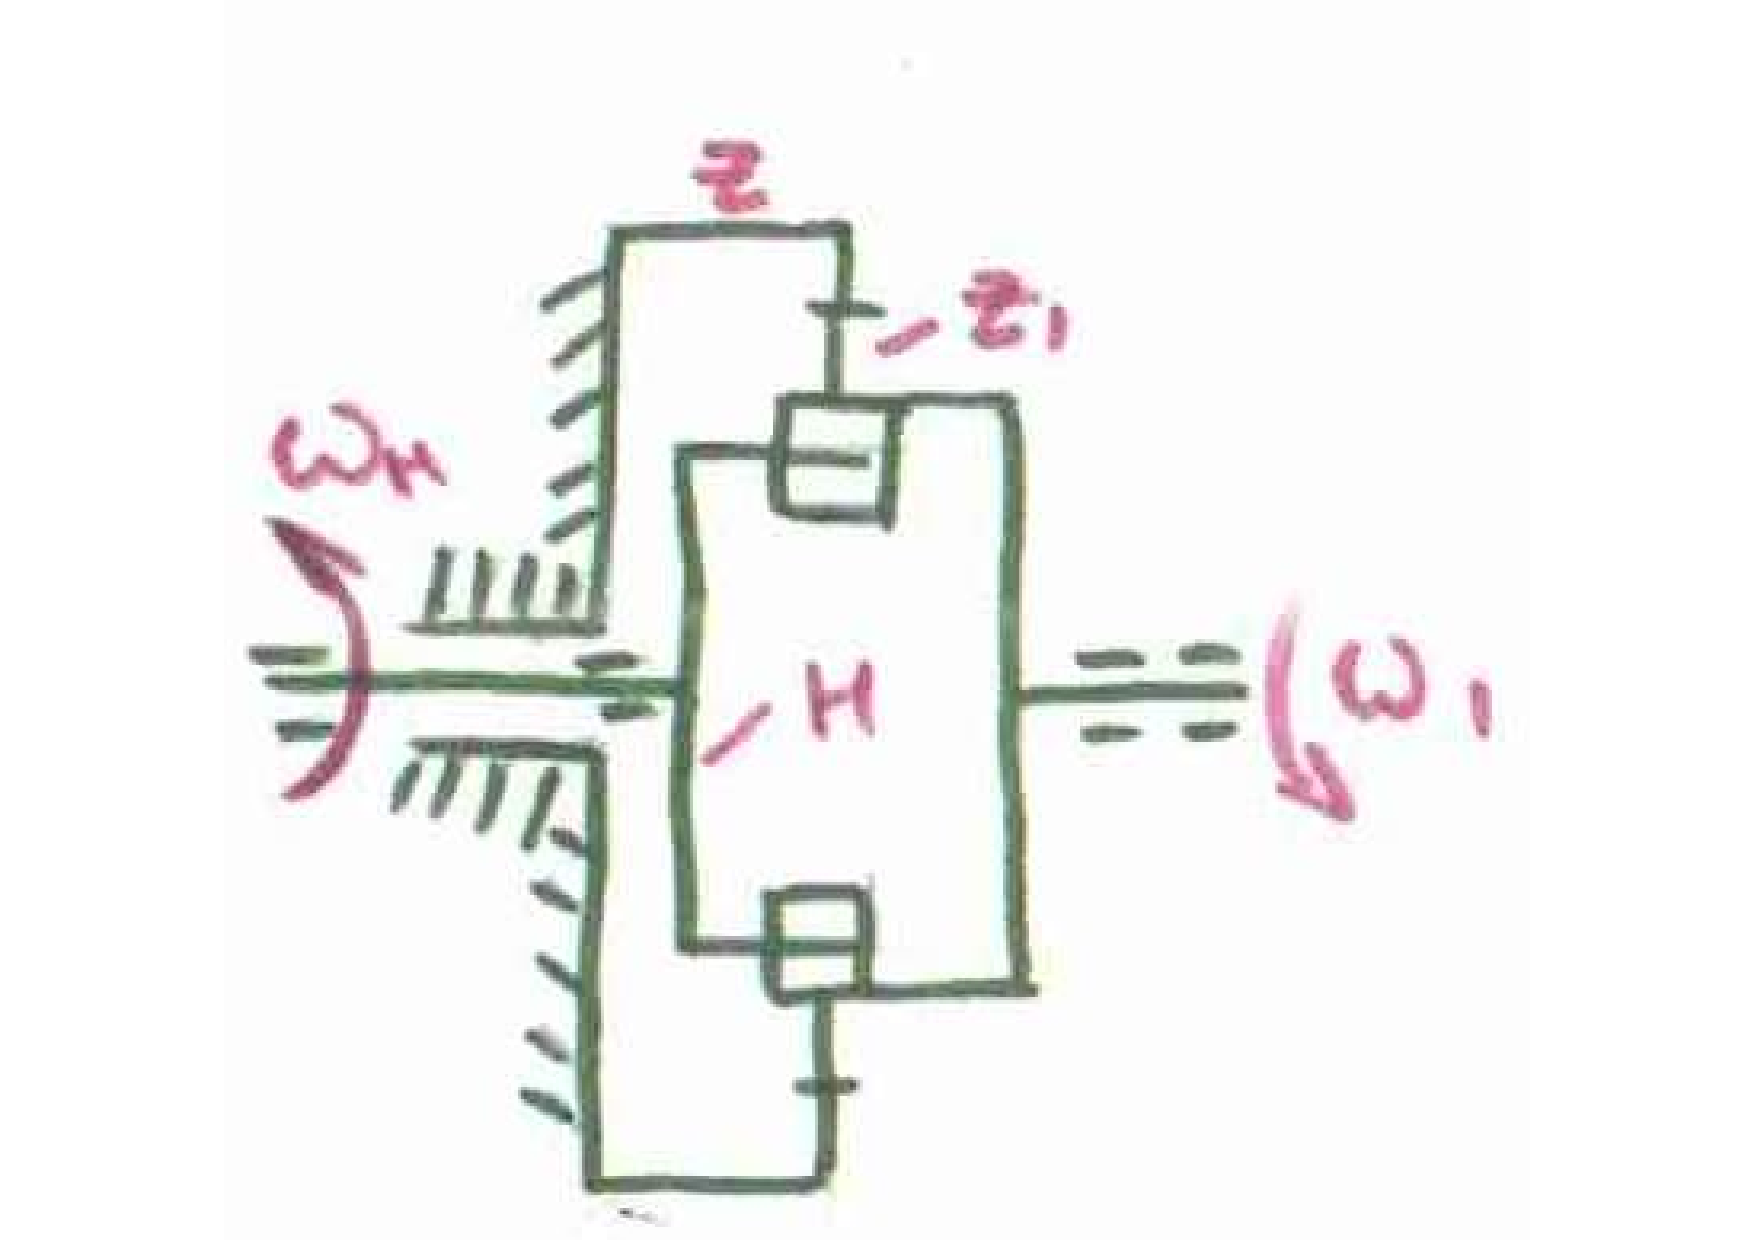
\includegraphics[width = 0.2\textwidth]{15_2}

\underline{Достоинства} 
\begin{enumerate}
	\item Выскоая нагрузочная способность т.к. в закцеплении всегда находятся 30-50\% зубьев
	\item Более высокая кинематическая точность в сравнии с обычными зумбчатыми редукторами, т.к большое кол-во зубьев одновеменно находятся в зацеплении и погрешность окружных шагов устраняется
	\item Работает сравнительно плавно и бесшумно
	\item $\eta = 80 .. 90 \%$
	\item Возможность передачи движения через герметичную стенку
\end{enumerate}
\underline{Недостатки}
\begin{enumerate}
	\item Специфические материалы гибкого колеса быстро изнашиваются
\end{enumerate}

\section {Сложные передачи. Планетарные передачи.}

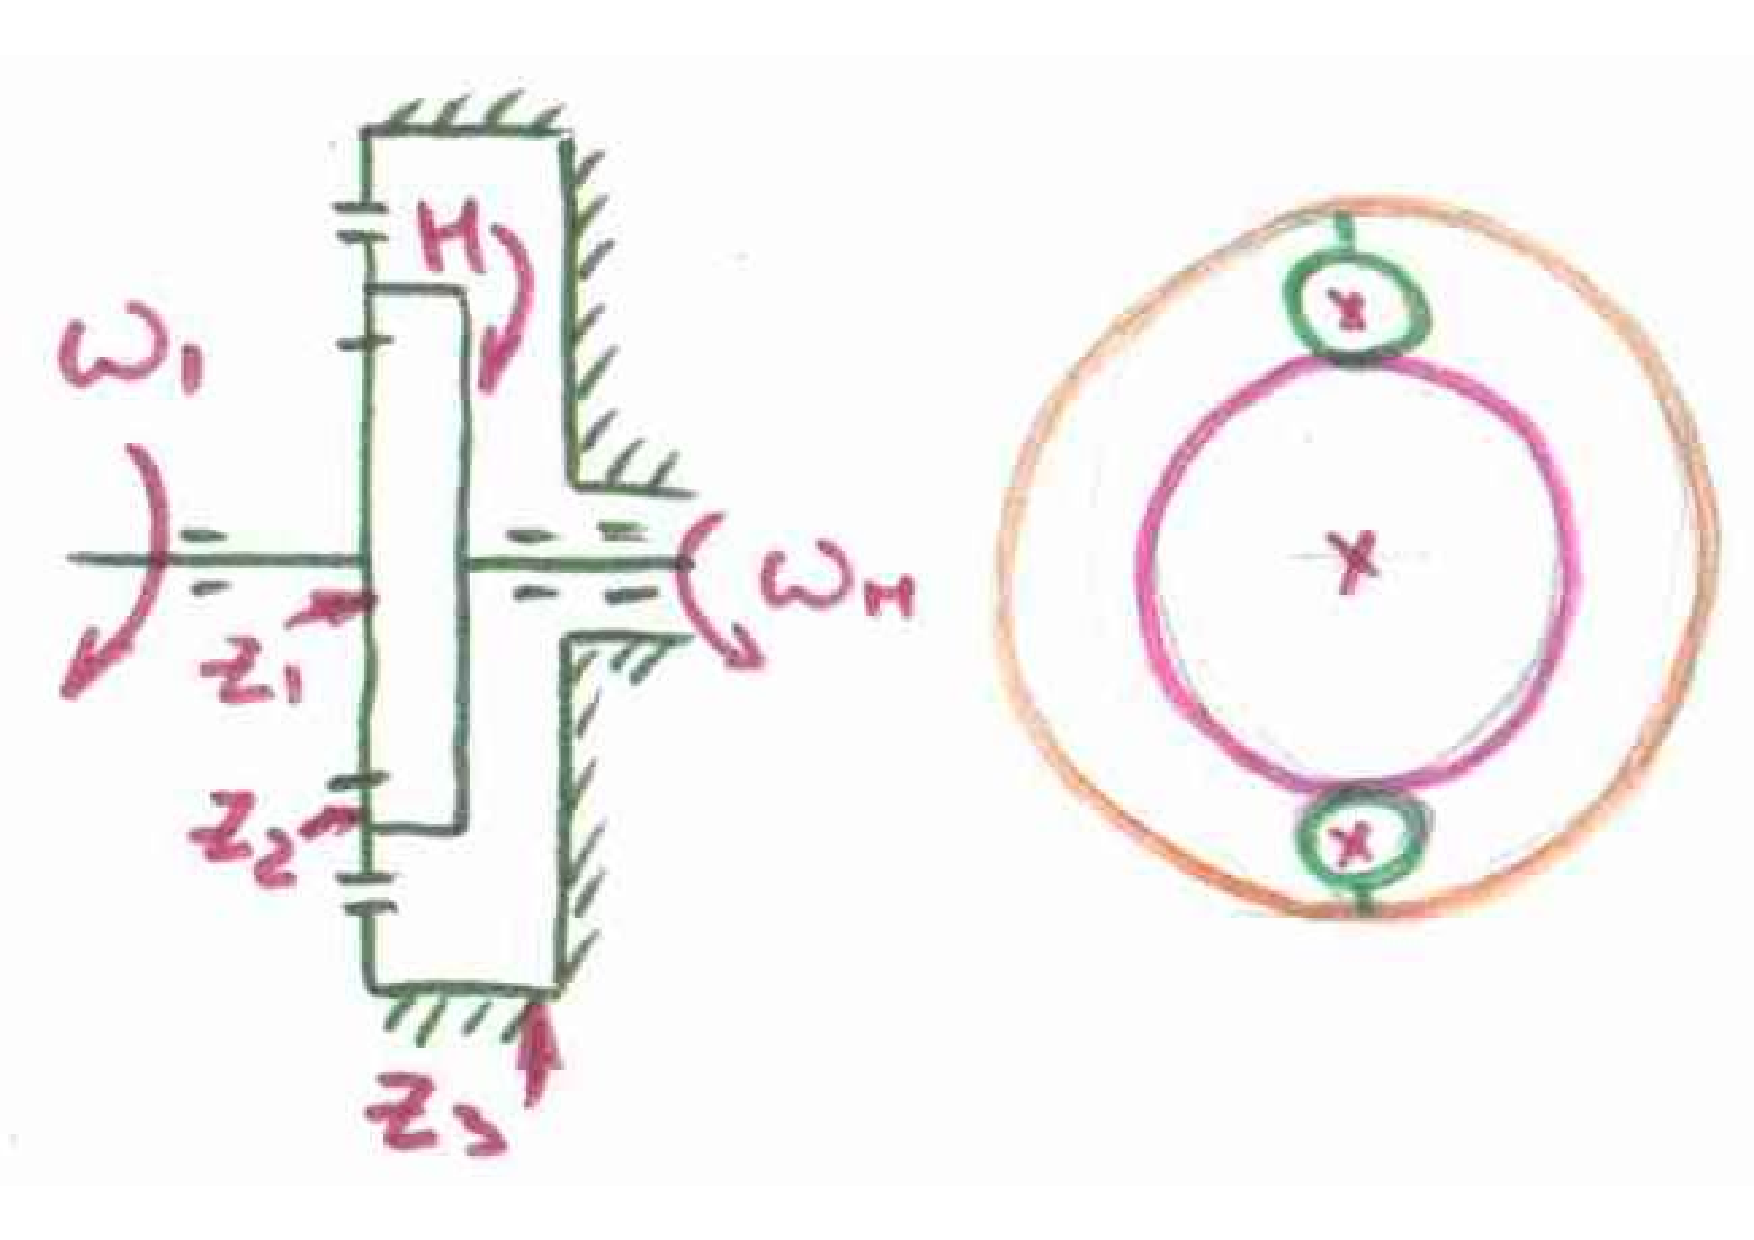
\includegraphics[width = \textwidth]{16_1}

\underline{Планетарными} называются передачи, состоящие из зубчаных колес и вращающихся звеньев, на которых располагаются оси зубчатых колес.

Звено на котором располагаются подвижные оси колес, нвызвается водило H, А зубчатые колеса с подвижными осями наз. сателитами. Колесо с неподвижной осью вращения $z_1$ называется солнечным. Неподвижное колесо $z_3$ наз. опорным (или короткой).

Расчет передаточного отношения планетарной передачи методами обращенного движения (Формула Смирнова-Виллиса).

\begin{tabular}{ccc}
	& Исходное & Обращенное\\
	солнечное колесо $z_1$ & $\omega_1$ & $\omega_1 - \omega_н$\\
	сателит $z_2$ & $\omega_2$ & $\omega_2 - \omega_н$\\
	водило H & $\omega_н$ & 0\\
	опорное колесо $z_3$ & $\omega_1$ & $- \omega_н$\\
\end{tabular}
$$
i_{1\:н} = \frac{\omega_1}{\omega_н}
$$
$$
i_{13}^{(н)} = \frac{\omega_1 - \omega_н}{- \omega_н}  = 1 - \frac{\omega_1}{\omega_н} = 1 - i_{1н}
$$
$$
i_{13}^{(н)} = \frac{z_3}{z_2} \left(- \frac{z_2}{z_1} \right) = - \frac{z_3}{z_1}
$$
\underline{Выбор числа зубьев}:
\begin{enumerate}
	\item Число зубьев дожно обеспечивать передаточное отношение $i_{1н}$
	\item Должно обеспечиваться условие соосности: $d_3 - d_1 = 2 d_2$, $z_3 - z_1 = 2 z_2$
	\item Должно обеспечиваться условие сборки: $\frac{z_1 + z_3}{K} = целое число$, k - число сателитов.
	\item Должно обеспечиваться условие соседства
\end{enumerate}
\underline{Достоинства}:
\begin{enumerate}
	\item Соостность входного и выходного вала
	\item Легкость получения большого передаточного отношения без существенного увеличения габаритов.
	\item В зацеплении могут находиться одновременно несколько пар зубьев зубчатых колес, что удменьшает нагрузку на пару зубчатых колес и уменьшает маодуль, а, следовательно, и уменьшает габариты.
	\item Наличие нескольких пар зацепления зубьев обеспечивает снижение погрешности кинематической и обеспечивает плавность хода
\end{enumerate}
\underline{Недостатки}:
\begin{enumerate}
	\item Резкий спад КПД при очень большом передаточном отношении.
\end{enumerate}

\section {Сложные передачи. Рядные передачи.}

\underline{Рядные передачи}

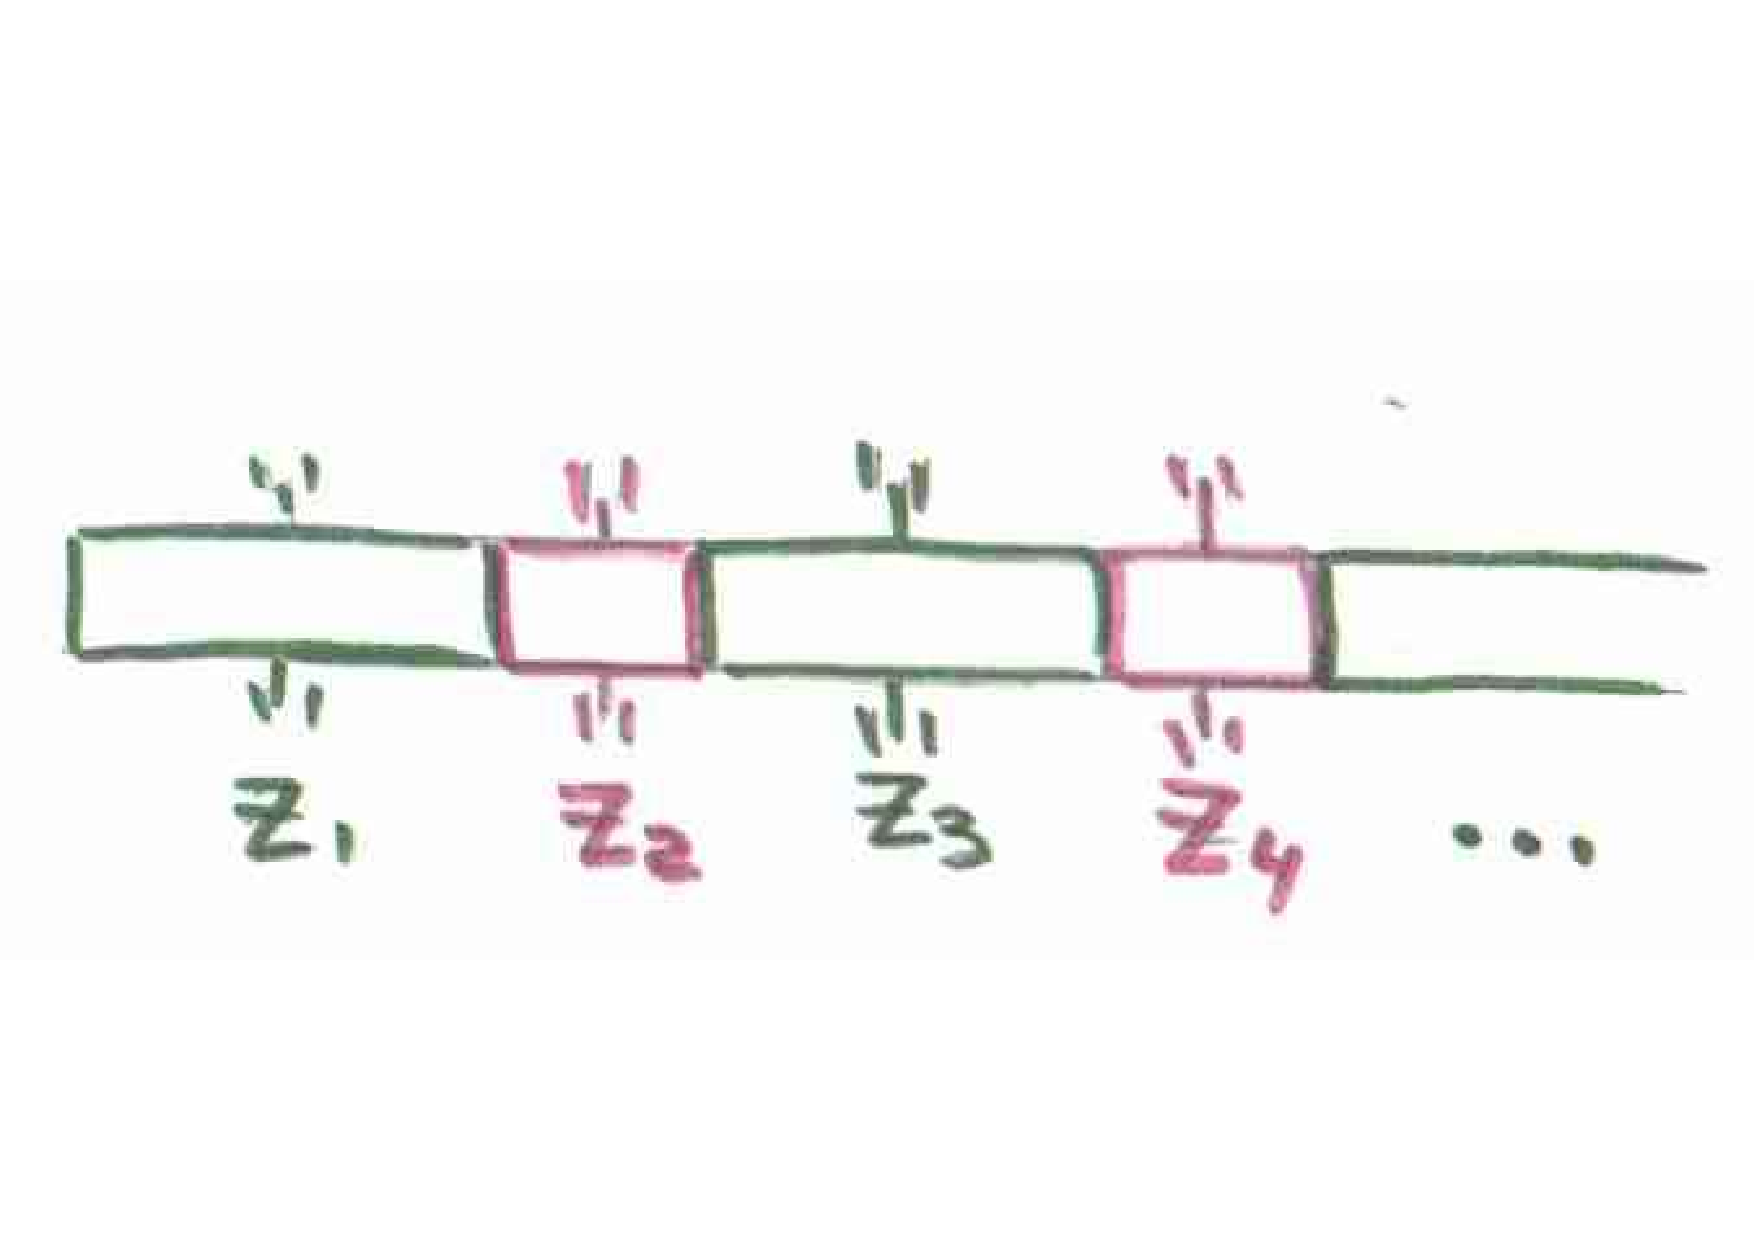
\includegraphics[width = 0.75\textwidth]{17_1}

$n$ -- количество зубчатых колес\\
$k$ -- количество зацеплений\\
$i_{1n} = (-1)^k \frac{z_n}{z_1}$\\
$\eta = \eta_{1\:2}\cdot\eta_{2\:3}\cdot\dots\cdot\eta_{i\:j}$\\
\underline{Применение:}
\begin{enumerate}
	\item Позволяют вписывать передачу в занные межосевые расстояния
	\item Когда необходимо согласовать вращение входного и выходного вала
	\item Служат для обхода препятствий внутри конструкций
\end{enumerate}
\underline{Достоинства:} 
\begin{enumerate}
	\item Возможность согласования валов на определенном межосевом расстоянии
	\item Возможность смены навпрления вращения передачи без пересчета передаточного отношения
	\item Возможноность обходения препятствий внутри конструкции
	\item Возможность снятия показаний с нескольких выходных валов
\end{enumerate}
\underline{недостатки:} 
\begin{enumerate}
	\item В передаточном отношении участвуют только первое и последнее зубчатые колеса, все остальные являются паразитными
	\item Относительно низкое КПД
	\item Большое кол-во промежуточных элементов
\end{enumerate}

\underline{Многоступенчатые передачи} 

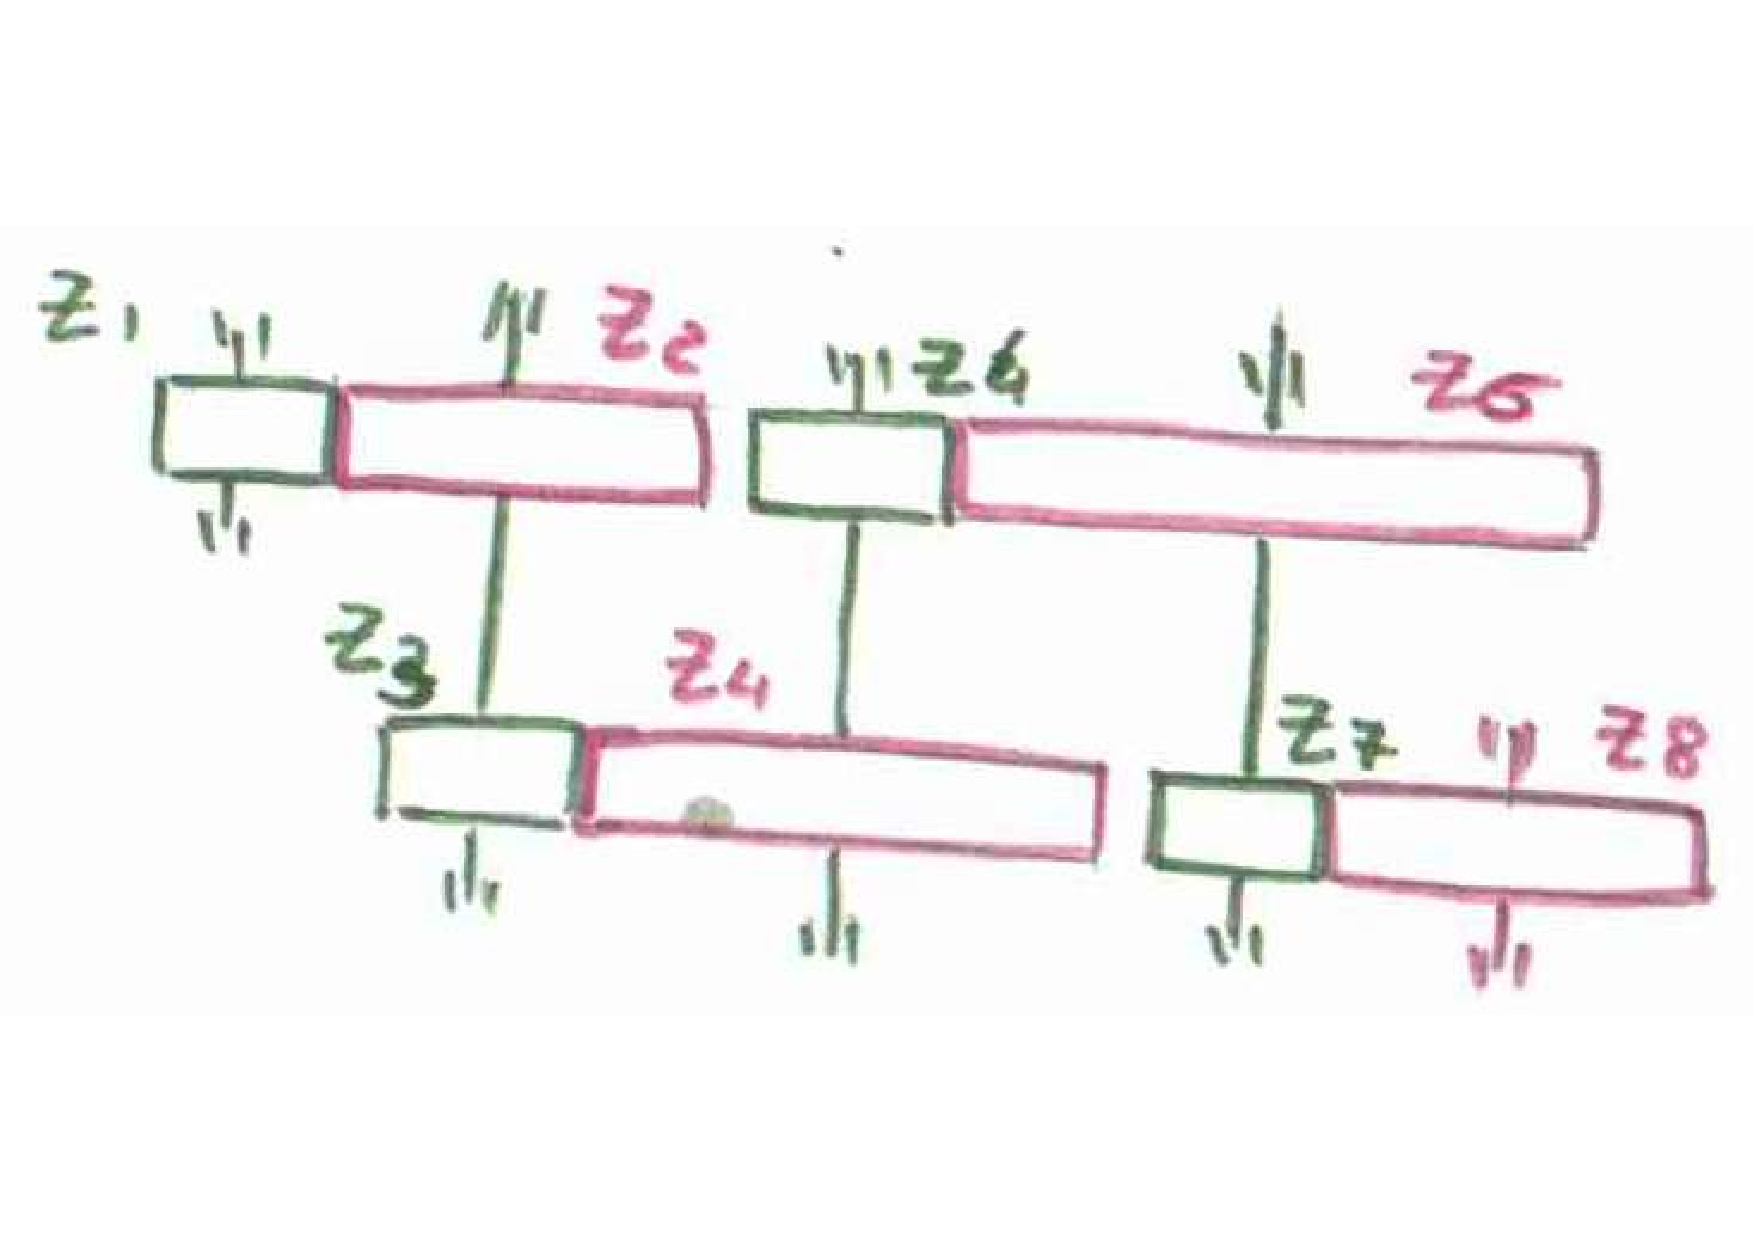
\includegraphics[width = 0.75\textwidth]{17_2}

$i_{1n} = (-1)^k \frac{z_2 \dots z_n}{z_1 \dots z_{n-1}} = i_{12} \cdot i_{34} \cdot \dots \cdot i_{(n-1)n}$\\
$\eta = \eta_{12} \cdot \eta_{34} \cdot \dots \cdot \eta_{(n-1)n}$\\

\underline{Применяются}, когда необходимо получить высокое пердаточное отношение
\underline{Достоинства:}
\begin{enumerate}
	\item Можно получить как очень большие передаточные отношения, так и очень маленькое
	\item Возможность снятия нагрузкис нескольких выходных валов при одном входном.
	\item Большое передаточное отношение при сравнительно маленьких габаритах.
	\item Простота расчета
	\item Простота сборки
\end{enumerate}
\underline{Недостатки:} 
\begin{enumerate}
	\item Резкий спад КПД при росте передаточного отношения.
\end{enumerate}

\section {Сложные передачи. Фрикционные передачи.}

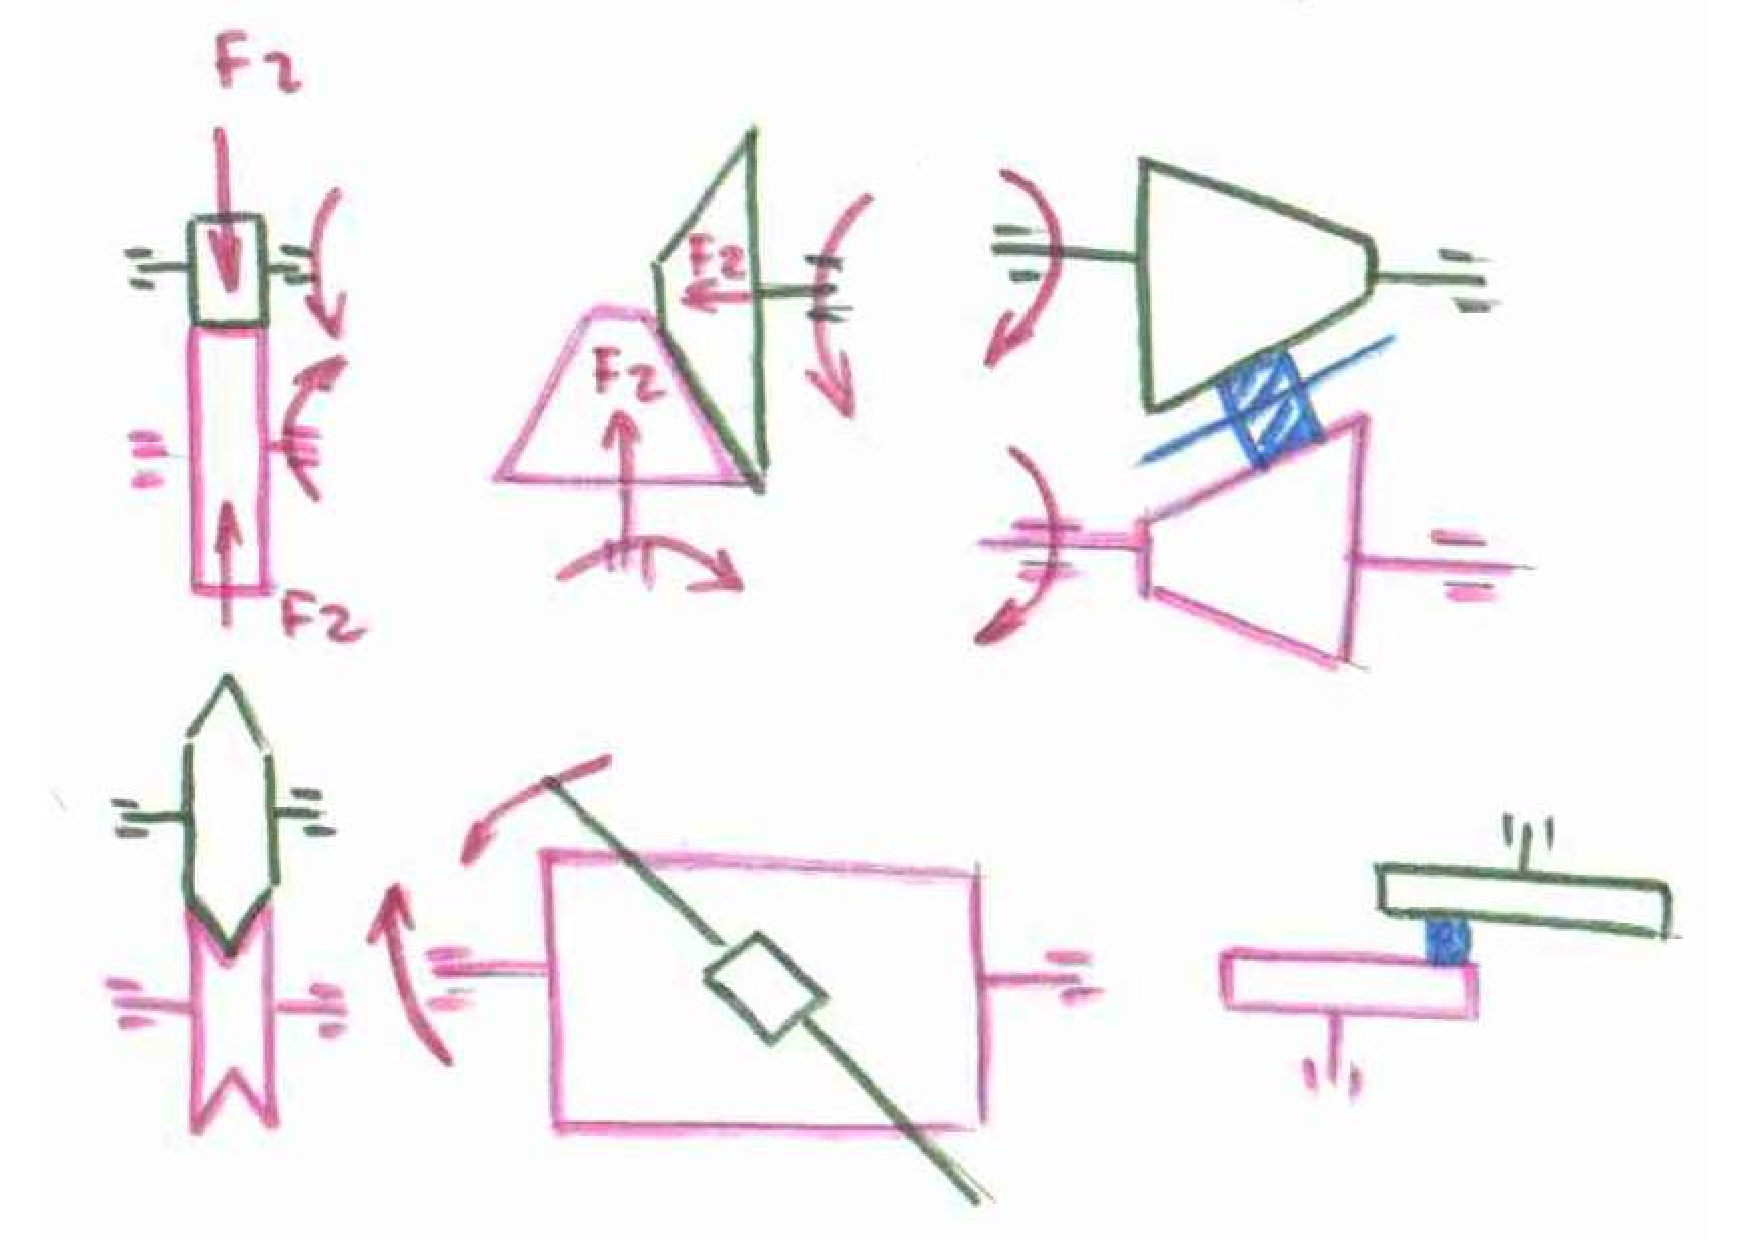
\includegraphics[width = 0.3\textwidth]{18_1}
\underline{Классификация:} 
\begin{enumerate}
	\item По взаимному расположени осей бывают:
	\begin{enumerate}
		\item Параллельные
		\item Пересекающиеся
		\item Скрещивающиеся
	\end{enumerate}
	\item По взаимному расположению контактов:
	\begin{enumerate}
		\item С внешним
		\item С внутренним
	\end{enumerate}
	\item По возможности варьирования передаточного отношеия:
	\begin{enumerate}
		\item С нерегулирумым передаточным отношением
		\item С регулируемым бесступенчатым передаточным отношением (вариаторы)
	\end{enumerate}
\end{enumerate}

\underline{Достоинства:} 
\begin{enumerate}
	\item Простота конструкции, изготовления, эксплуатации
	\item Легкость бесступенчатого варьирования передаточного отношения
	\item Легкость включения и переключения
	\item Сравнительная бесшумность в работе
	\item Возможность самозащиты от поломок.
\end{enumerate}

\underline{Недостатки:}
\begin{enumerate}
	\item Необходимость введения специальных нажимных устройств, вызывющих возникновения больших осевых сило в опорах
	\item Невозможность получения точного передаточного отношения из-за проскальзывания.
	\item Повышенный износ
\end{enumerate}

\underline{Геометрические и кинематические соотношнеия:} 

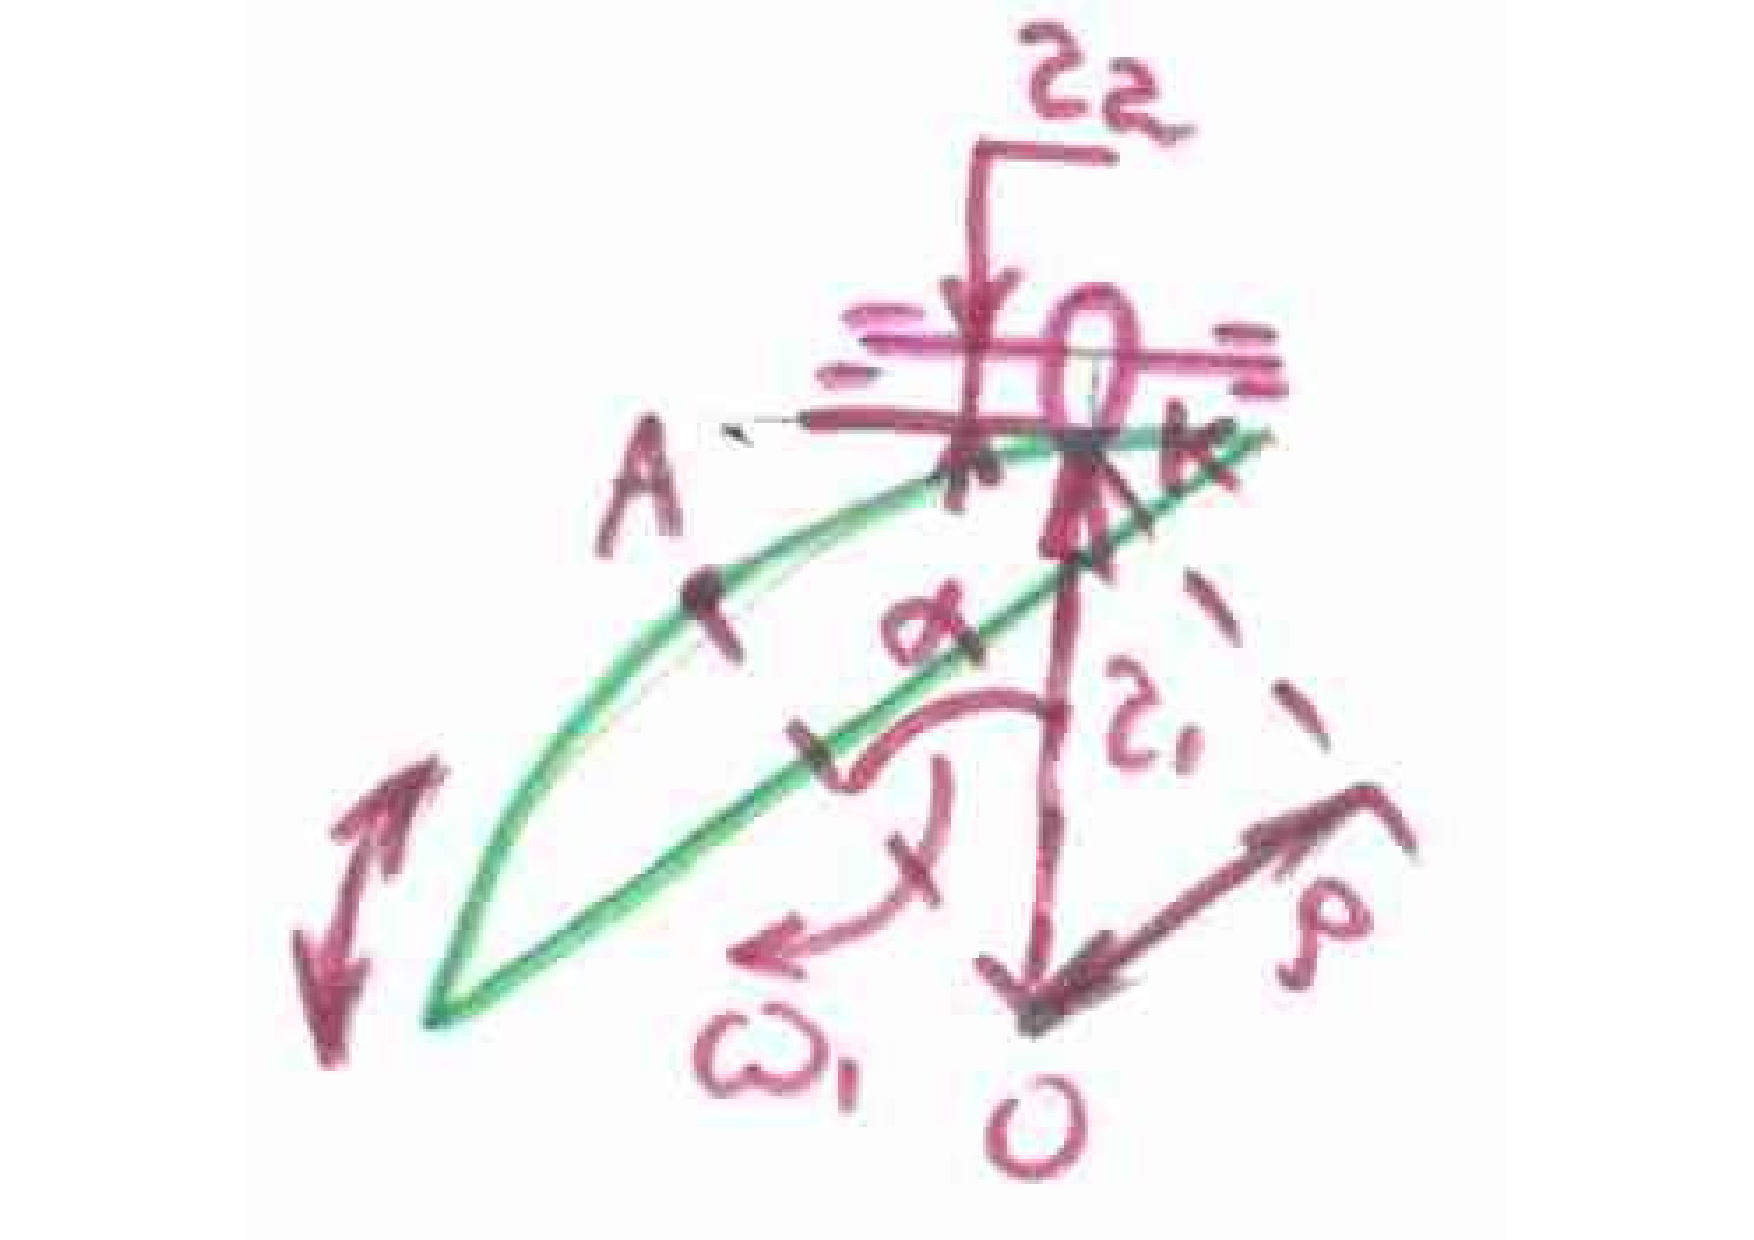
\includegraphics[width = \textwidth]{18_2}
\begin{enumerate}
	\item $V_1 = V_2$
	\item $ \frac{ \omega_1 d_1}{2} = \frac{\omega_2 d_2}{2} $
	\item $i_{1\:2} = \frac{\omega_1}{\omega_2} = \frac{d_2}{d_1} $
	\item $\rho = r_1 \sin {\alpha}$
	\item $\omega_1 \cdot \rho = \omega_2 r_2$
	\item $ \frac{\omega_1}{\omega_2} = \frac{r_2}{r_1 \sin{ \alpha}} $
	\item $ i_{1\:2} = \frac{r_2}{r_1 \sin { \alpha}} $
\end{enumerate}

Если $ \alpha \to 0$, тогда $i_{1\:2} \to \infty$, $\omega_2 \to \infty$
\section {Упругие чувствительные элементы.}

УЧЭ служат для преобразования измеренного давления или силы в какие-либо механические перемещения. К ним относятся пружины,
мембраны, мембранные коробки, гофрированные трубки, тубчаные сифоны (сильфоны???)

Характеристика упругого чувствительно элемента --- зависимость между его прогибом (ходом) и вызывающей этот прогиб нагрузкой.

Пружины делятся:
\begin{enumerate}
	\item По форме:
	\begin{enumerate}
		\item Прямые
		\item Изогнутые
		\item Плоские
		\item Спиральные
		\item Винтовые
	\end{enumerate}
	\item По назначению:
	\begin{enumerate}
		\item Силовые (аккумуляторы энергии)
		\item Измерительные (УЧЭ)
		\item Для соединения деталей
	\end{enumerate}
\end{enumerate}

\section {Упругие чувствительные элементы. Основные формулы для расчета.}

\begin{enumerate}
	\item Допускаяемая нагрузка: $P_{max} = \frac{\pi d^3}{8 \cdot D_0} $
	\item Максимальное анпряжение: $\tau_{max} = k \frac{8 P_{max} D }{\pi d^3} \le [\tau_{кр}]$
	где $k$ -- коэфициент зависящий от индекса пружины:
	\item Индекс пружины: $C = \frac{D_0}{d} $, $C = 4 \dots 10, d > 0.5 мм$, $C = 6 \dots 16, d \le 0.5 мм$
	для приборных пружин $c = 8 \dots 12$
	\item $k = \frac{4 C - 1}{4 C - 4} $, при $C > 10, k = 1$
	\item Диаметр проволоки: $d \ge \sqrt[2]{ \frac{8 P_{max} C K}{n [\tau_{F_p}]} }$
	\item Осевое перемещение: $f = \frac{8 D_0^3 P_{max} n}{G d^4} = \frac{8 C^3 P_{max} n}{G d } $
	\item Жесткость пружины: $K = \frac{G D^4}{8 n D_0^3} $
	\item Длина развернутой проволоки: $L = \frac{\pi D_0 n}{\cos{ \alpha}} $
\end{enumerate}

\section {Упругие чувствительные элементы. Расчет винтовой пружины.}
%\inludegraphics[width = \textwidth]{21\_1}

Определим размеры винтовой пружины сжатия при установке ее в прибор.
Пусть даны $P_{min}, P_{max}, F_{рабоч}$, материал прволоки, $\sigma_{B}, \alpha$
\begin{enumerate}
	\item $ \frac{f_{min}}{f_{раб}} = \frac{P_{min}}{P_{max} - P_min} \to $
	$f_{min} = \frac{P_{min} * f_{раб}}{P_{max} - P_{min}} $\\
	$f_{max} = f_{min} + f_{раб}$
	\item $d \ge \sqrt[2]{ \frac{8 P_{max} C K}{\pi [\tau_{кр}]} }$, где $[\tau_{кр}] = \frac{\sigma_{B}}{n_т}$,
	$C = \frac{D_0}{d } $,
	$K = \frac{4 C - 1}{4 C - 4} + \frac{0.615}{C} $
	
	Согласно ГОСТ 9389-75 выбираем ближайшее $d$

	$D_0 = d \cdot C$ -- средний диаметр\\
	$n = \frac{1}{8} \frac{G f_{max} d }{P_{max} C^3} $ -- количество витков\\
	$n_0 = n + 2$\\
	$L = \frac{\pi \cdot D_0 \cdot n_0}{\cos{ \alpha}} $
\end{enumerate}
\section {Червячные передачи. Расчет сил и моментов в червячной передаче.}



\section {Винтовые передачи. Классификация. Назначение. Достоинства и недостатки}

Передача винт-гайка \underline{предназначена} для преобразования вращательного движений в поступательное
\underline{Классификация:}
\begin{itemize}
	\item Кинематическая
	\item Силовая
\end{itemize}

Основные детали -- винт в виде цилиндра с наужной резбой и гайка в виде кольца с внутренней резьбой

\underline{Достоинства}
\begin{enumerate}
	\item Простота конструкции
	\item Относитлеьно высокое передаточное отношение
	\item Эффект самоторможения
	\item Высокая точность
\end{enumerate}
\underline{Недостатки:} 
\begin{enumerate}
	\item Высокое трение $\to$ быстрый износ
	\item Низкий КПД
\end{enumerate}

\underline{Виды преобразования:} 

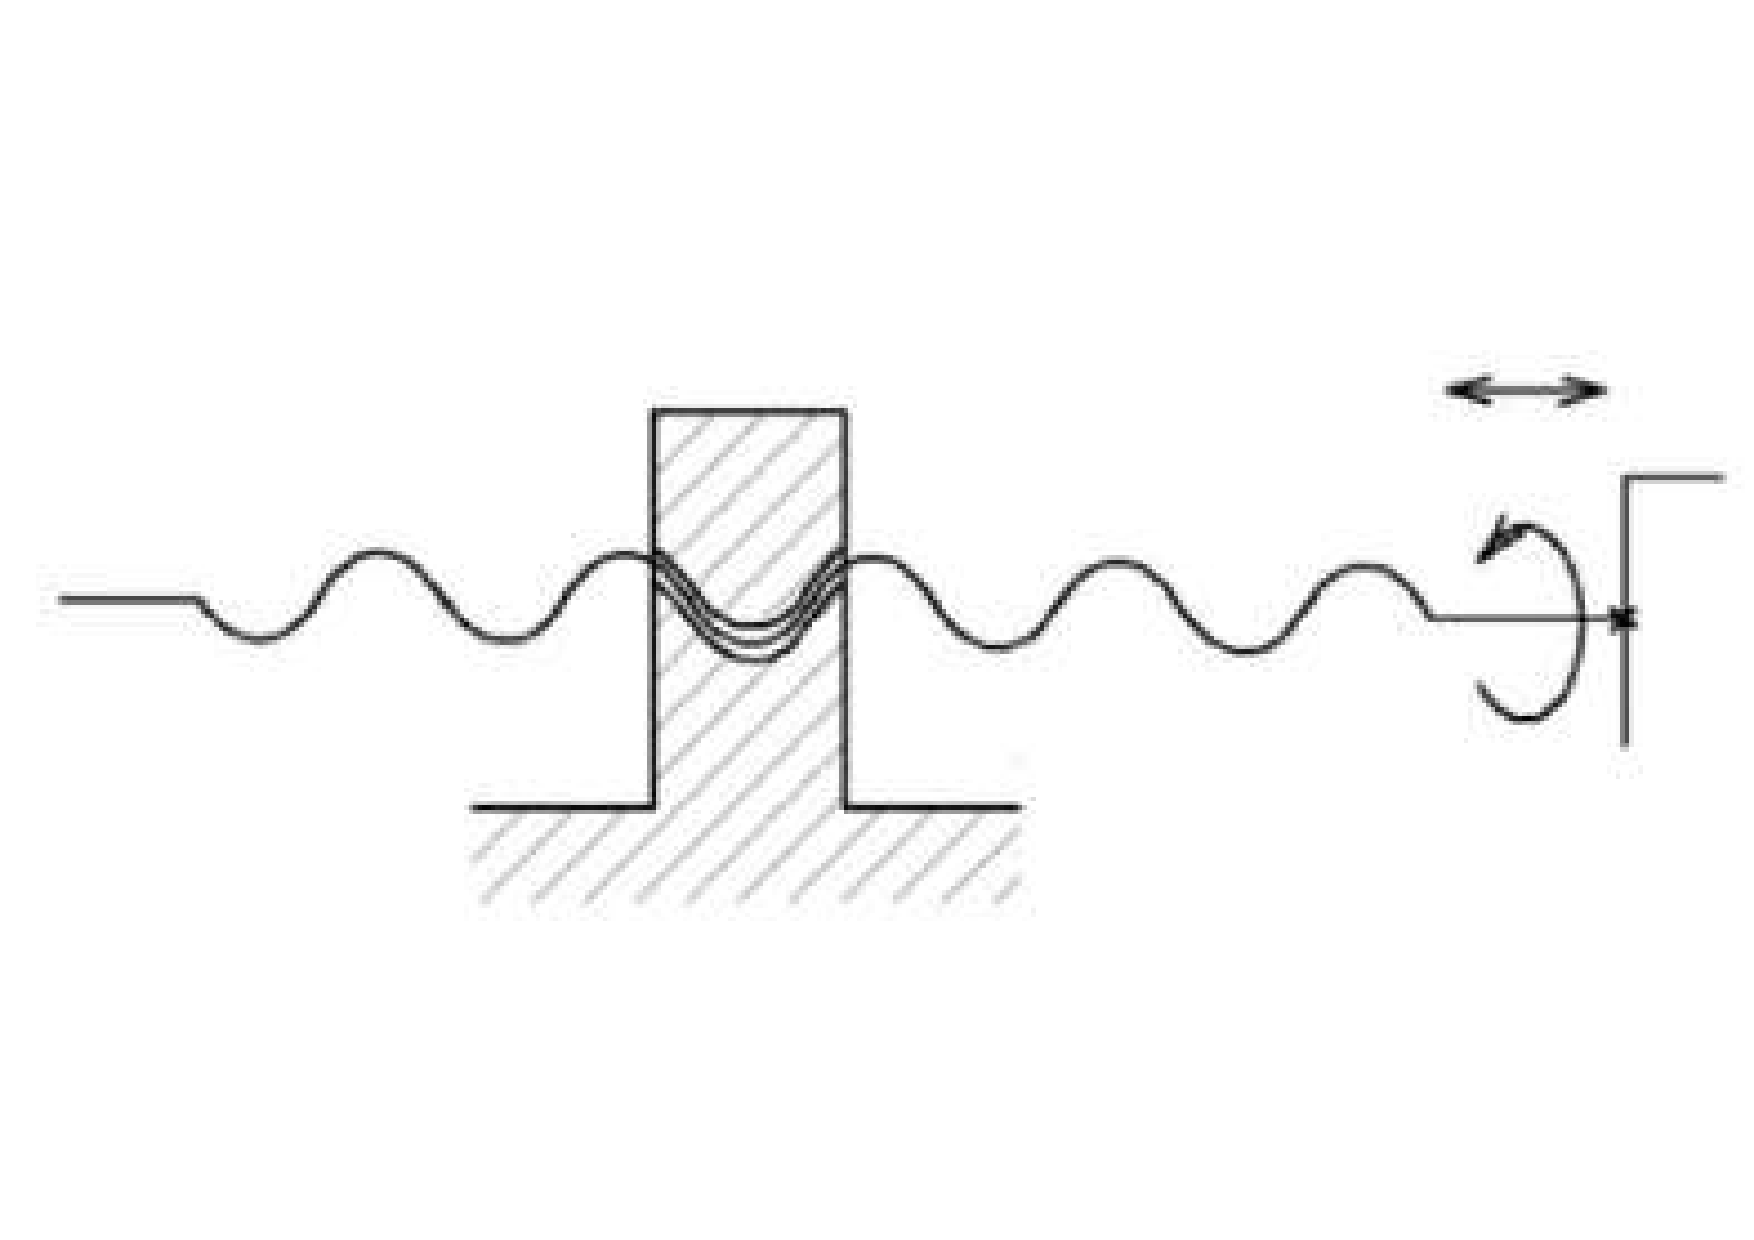
\includegraphics[width = 0.2\textwidth]{23_1}
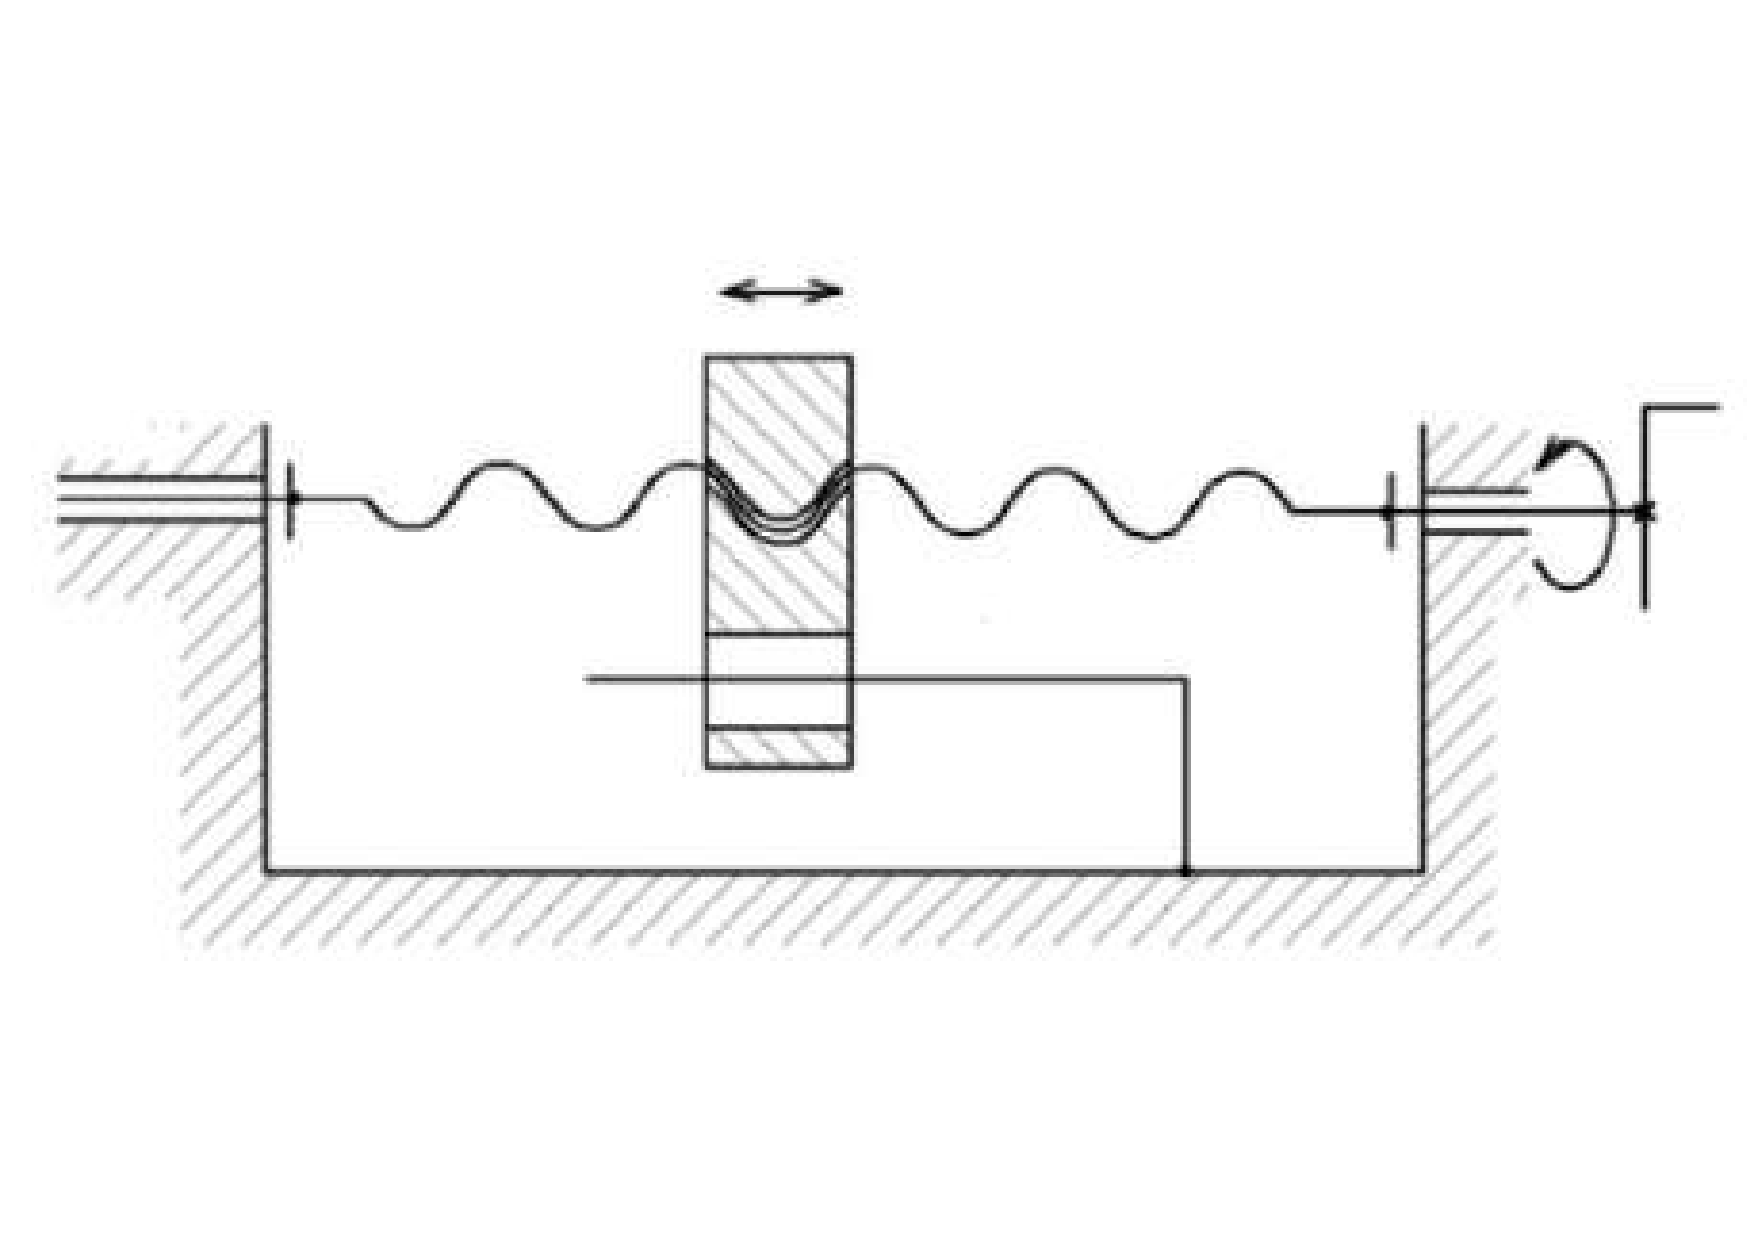
\includegraphics[width = 0.2\textwidth]{23_2}
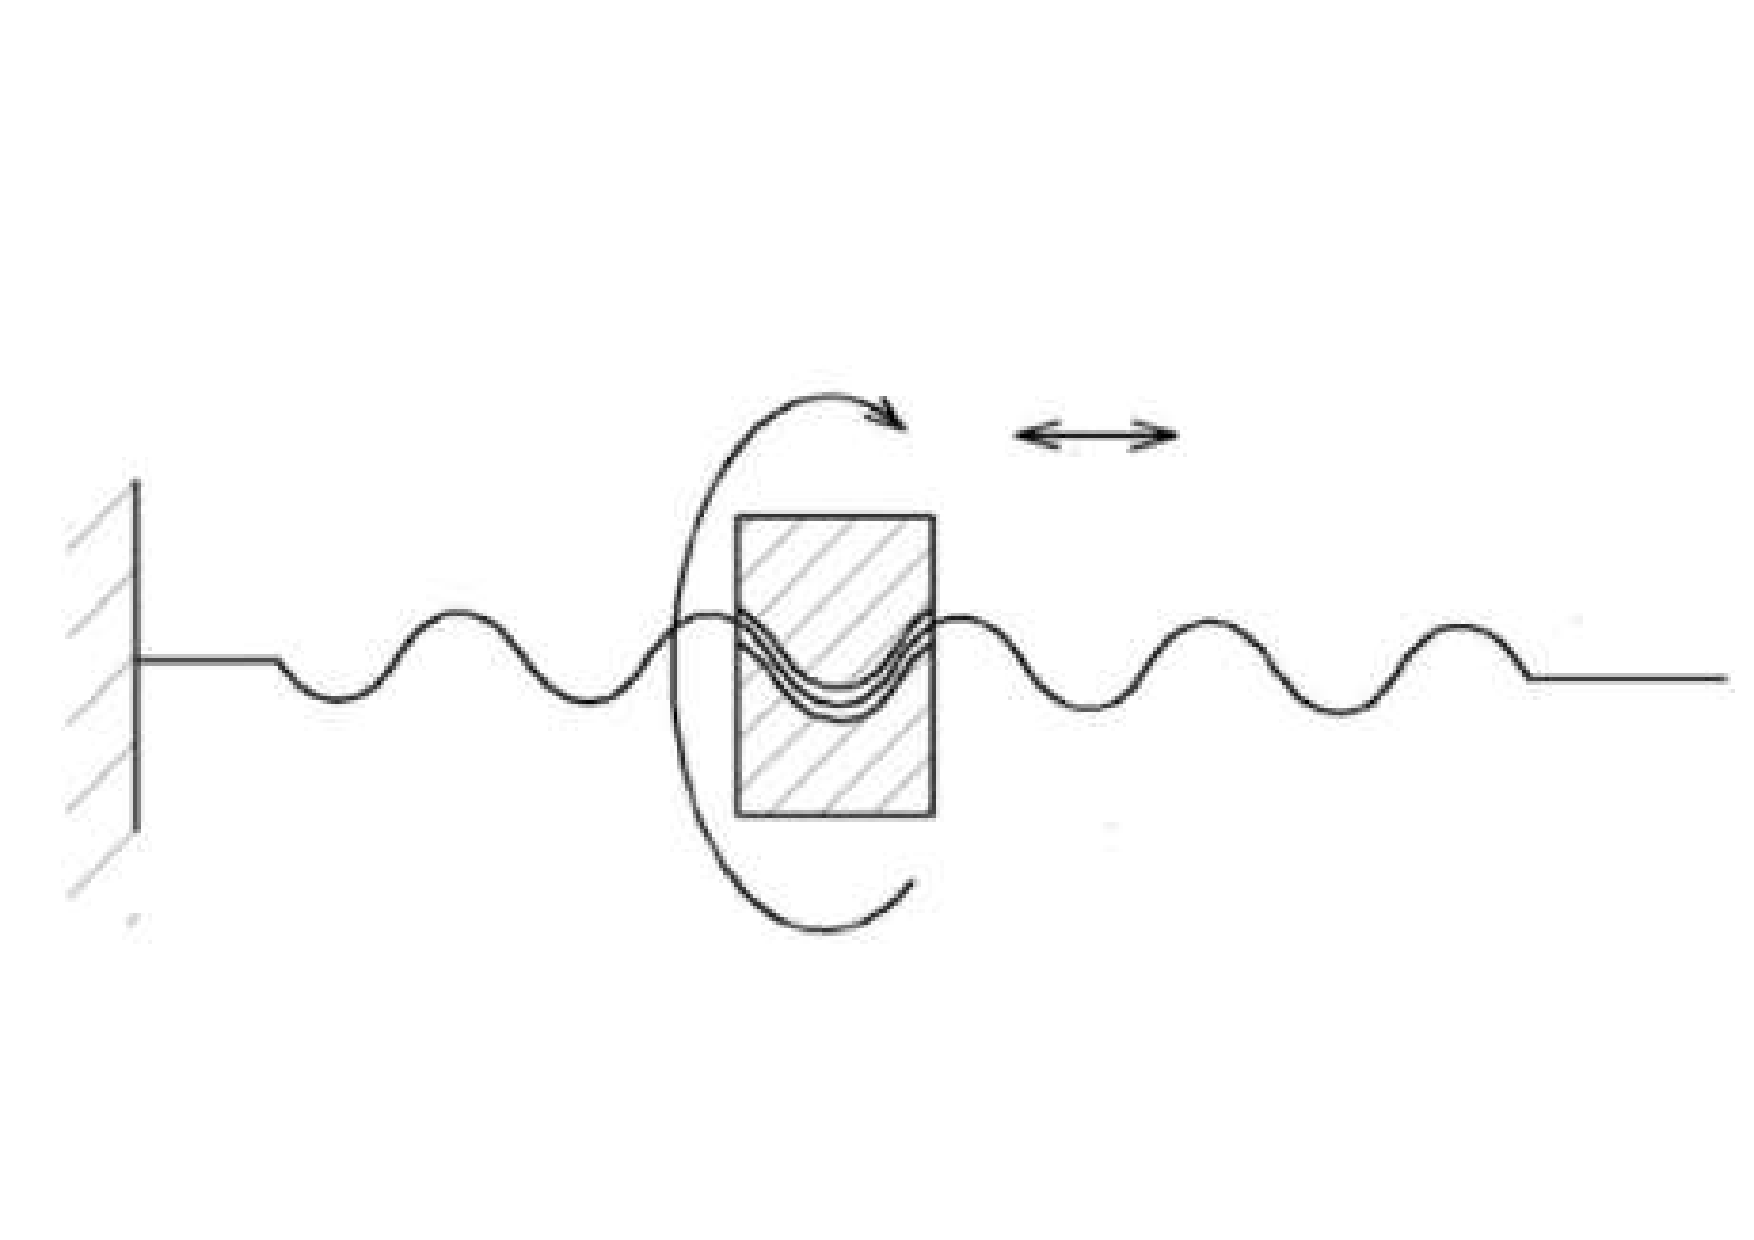
\includegraphics[width = 0.2\textwidth]{23_3}
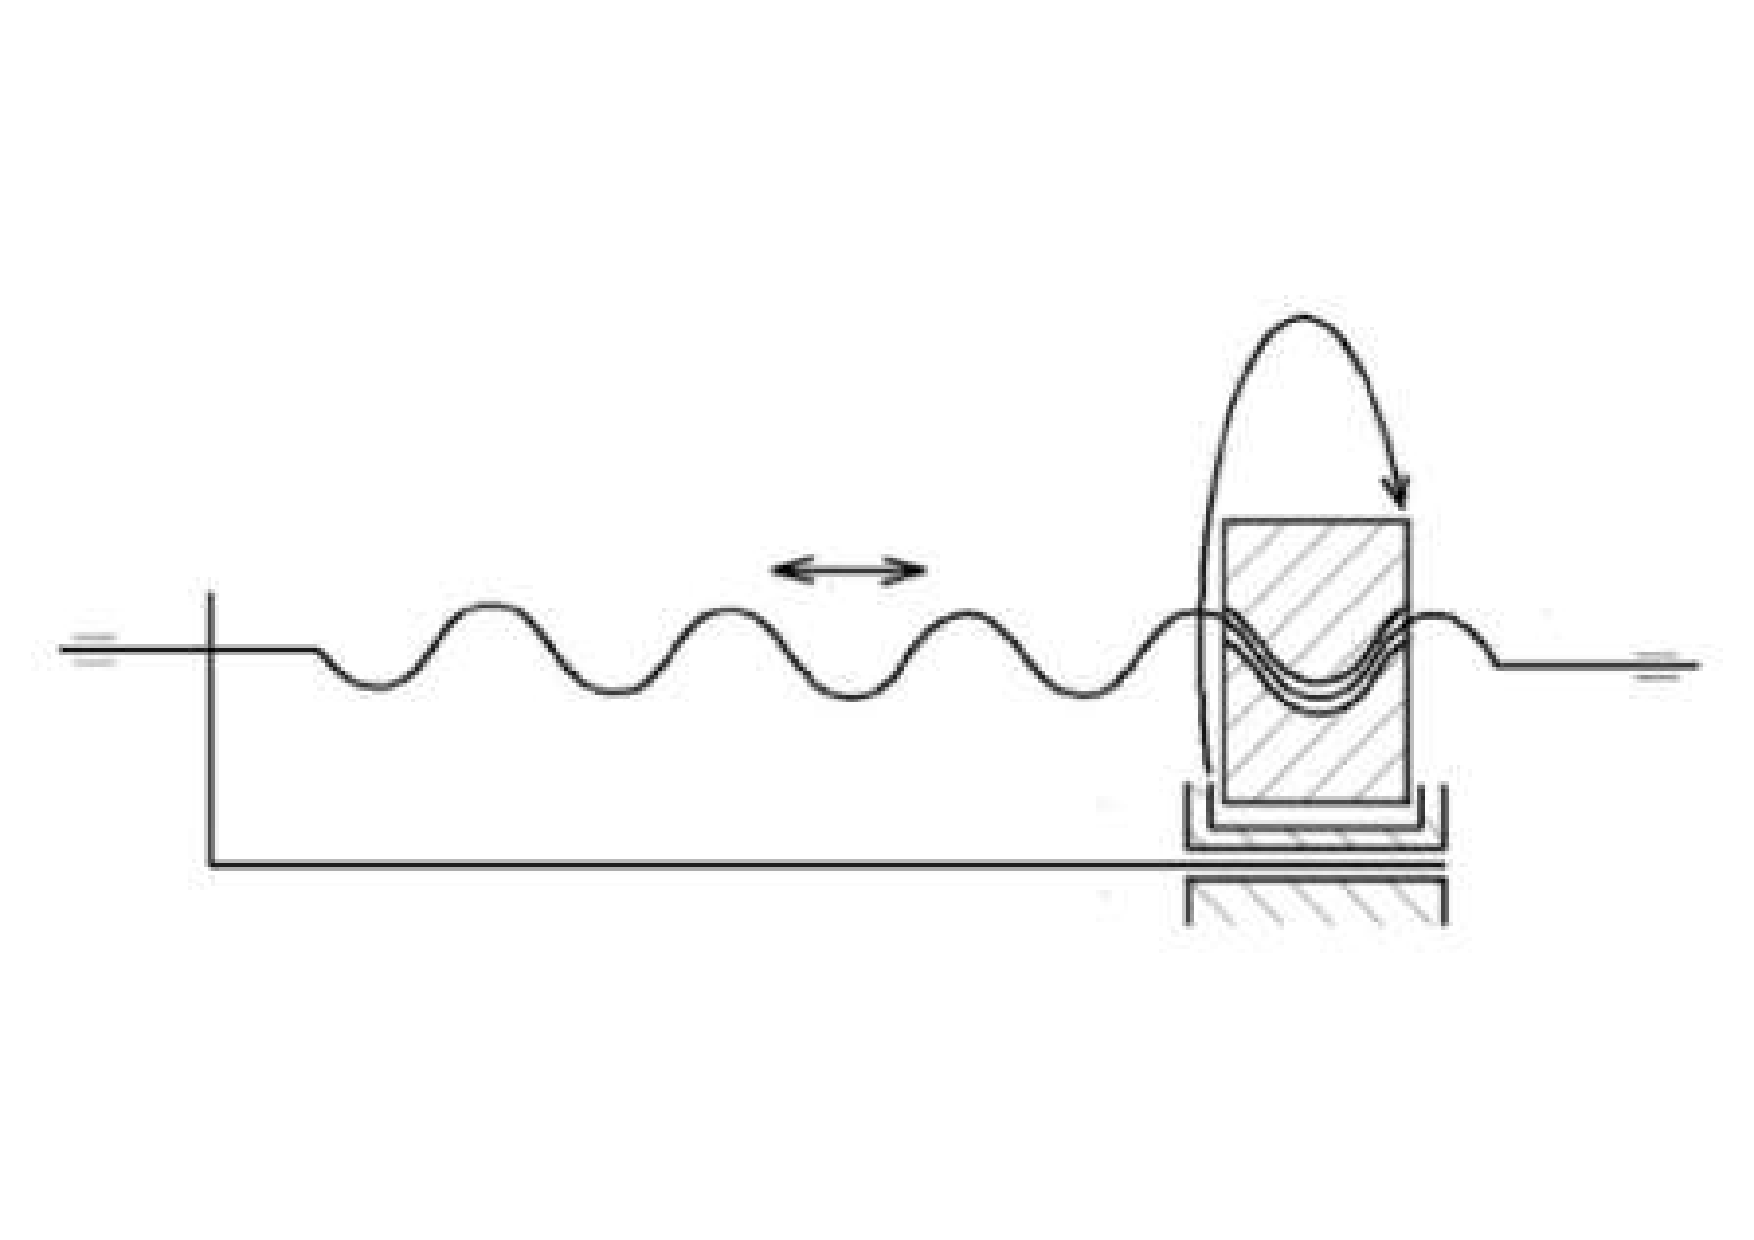
\includegraphics[width = 0.2\textwidth]{23_4}
\end{document}
